\chapter{Software Development in ROS2}\label{c:ros}

Robotic systems have emerged into several scenarios, where its usage ranges between basic processes automation, up to full performance over critical tasks, consequently causing the complexity increase in these domains. 

Due to the wide variety of robotic hardware presented in multiple domains, concerning about software development is rather difficult \cite{cousins2011exponential}. The reuse of code is non-trivial, and therefore, large-scale development is rendered untenable. The Robotic Operating System (ROS) presents itself as a middleware system, created to facilitate robotic system development in large scale.

In ROS, software flexibility was prioritized above all else, meaning that values like security were disregarded. Thus, ROS-based applications tend to face increased security risks, related to the exposure of the whole robotic network. Due to the scale and scope of the robotics growth, security insurance must be addressed as a developing priority \cite{diluoffo2018robot, kim2018security}.

The upgraded version of ROS, Robot Operating System 2 (ROS2), presents itself as a framework for developing robotic systems, supported by the Data Distribution Service (DDS) standard. Multiple middleware implementations are built over this standard, which provides numerous DDS-based specifications as well as valuable Quality of Service (QoS) transport parameters.

The DDS-Security specification \cite{dds-s} aims to supply multiple plugins regarding the security domain. Consequently, ROS2 yields a wider command toolset compared to the former version of ROS, as they bring forth to a toolset, the Secure Robot Operating System 2 (SROS2) toolset, concerning the security functionality that DDS-Security plugins offer.

This chapter introduces necessary background information over the major concepts on which this thesis rests. First, it is presented a detailed introduction to the concepts around Robot Operating System (ROS), as well as the evolution approach that ROS faced towards providing security to its deployed systems. Regarding this goal, Data Distribution Service (DDS) and its integration on Robot Operating System 2 (ROS2) must be contextualized beforehand.


\section{Architecture Considerations}

The Robot Operating System was created by a collaborative open-source community, that has undergone rapid development \cite{cousins2011exponential} to contribute in the advancement of cyber physical systems. It was purposefully designed to be a development enhancer for the realm of robotic applications \cite{diluoffo2018robot, intro-ros}.

Fundamentally, ROS is a middleware, as it provides a custom serialization format, a custom transport protocol as well as a custom central discovery mechanism, presenting itself as a distributed layer between the top application layer and the operating system layer. 

ROS was designed to provide as much as modularity and composability to the application layer as possible \cite{casini2019response}, allowing ROS applications to be built over several software modules, as independent computing processes called \textit{nodes}. These compose together to fulfill the deployment characteristics of the corresponding robot \cite{maruyama2016exploring}.

\subsection{Former Architecture}

The Robot Operating System architecture is based on a hybrid peer-to-peer implementation, where network communication is done over message-passing through a publish-subscribe pattern. The architecture emphasized on approaching communication through a centralization perspective. It relied on the explicit implementation of a \textit{Master node}, that controlled every aspect of the communication establishment. Consequently, every information exchange within the network had to go through this master.

Formerly, due to the sheer wide capabilities controlled by the master, this centralization approach was duly valorized. It naturally fits the purposes of a research tool, as it is simpler to monitor and analyze the system behaviour. However, because it is strongly reliant on the master node's availability, this communication architecture does not scale effectively, making it unsuitable for safety-critical or real-time applications. If the master fails, the entire system fails, representing a single point of failure and a huge performance bottleneck.

\begin{figure}[H]
  \centering
  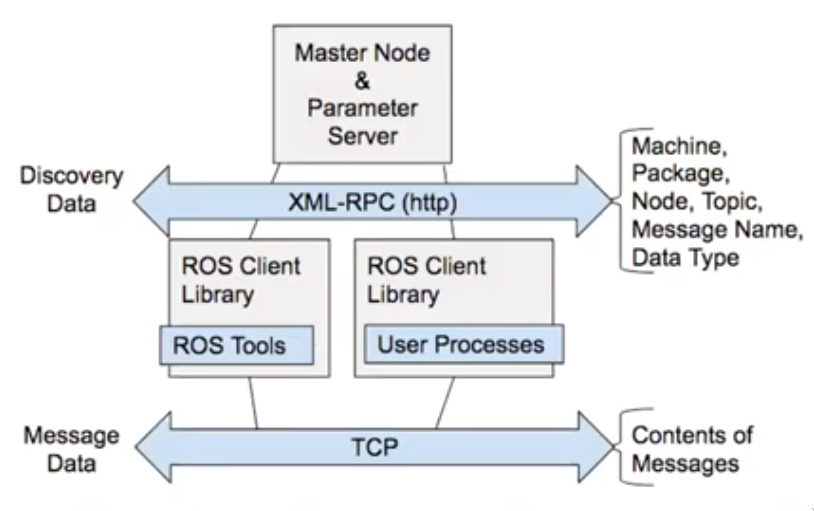
\includegraphics[width=0.6\linewidth]{images/former-ros1-architecture.png}
  \caption{Robot Operating System architecture.}
  \label{fig:ros1-architecture}
\end{figure}

Many research communities tried to fix these real-time issues by proposing potential solutions, while supporting the same architecture design. Unfortunately, fell short of meeting the requirements of real-time applications. It became clear to the ROS community that the framework had architectural limitations that could not be rearranged using the same design approach \cite{maruyama2016exploring}.

The \textit{Robot Operating System 2} comes as a complete refactoring of ROS, with the aim of increase the framework's real-time capabilities, by allowing the development of time-critical control over ROS, as it moves away from the former architectural design towards the implementation of an external middleware that can support the production needs of the outgrowing robotic systems \cite{kim2018security, casini2019response}.

\subsection{Data Distribution Service}

The \textit{Data Distributed System} (DDS) \cite{3} is an \textit{Object Management Group} (OMG) middleware standard. The standard was developed to address the demand for enhanced interoperability across different vendors' middleware frameworks, directly addressing data communication between nodes that belong to a \textit{publish-subscribe} communication architecture, for real-time and embedded systems. 

A communication middleware aims to ease the complexity behind creating and maintaining communication architectures. It is responsible for handling relevant aspects like network configuration, communication establishment, data sharing and low-level details. As a result, system developers can mainly focus on their applications purposes, rather than concerning about information moving across levels \cite{dds-what-is}. 

DDS uses the \textit{Data-Centric Publish Subscribe} (DCPS) model as its communication model approach. DCPS is based on a publish-subscribe pattern, where the \textit{data-centric} messaging technique is implemented. It conceptually creates a virtual \textit{Global Data Space}, acessible by any DDS-based application, where data is properly delivered to the applications which quest for it, saving bandwith and processing power \cite{3, pardo2005introduction}. A \textit{domain participant} enables an application to participate in the \textit{Global Data Space}, either as a \textit{publisher} or as a \textit{subscriber}, according to their role on data exchange \cite{maruyama2016exploring, alaerjan2017modeling, dcps-rtps}. 

\begin{figure}[H]
    \centering
    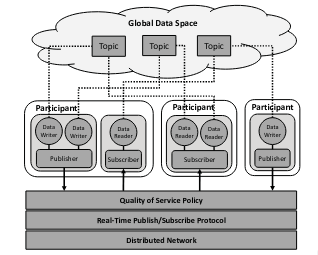
\includegraphics[width=0.5\linewidth]{images/dcps-model.png}
    \caption{DDS architecture: DCPS model with RTPS. Extracted from \cite{maruyama2016exploring}.}
    \label{fig:dcps-model}
\end{figure}

To properly address the data transportation through physical network, DDS offers a wire specification protocol called \textit{Real-Time Publish-Subscribe Wire Protocol} (RTPS) \cite{rtps}, providing automatic discovery between participants. This protocol also works under a publish-subscribe policy over best-effort transports, where data transmission between endpoints is handled \cite{yun2017data}. RTPS allows multiple applications, that could differ on their used DDS implementations, to interoperate with each other as network domain participants \cite{dcps-rtps, alaerjan2017modeling}.

Furthermore, RTPS was designed to employ \textit{Quality of Service} (QoS) profiles, which allow for the specification of various transport policies, formerly not covered by DDS. This approach offers flexibility over communication configuration and development versatility, allowing the developer to specify whatever QoS satisfies its system's communication needs \cite{alaerjan2017modeling, diluoffo2018robot, maruyama2016exploring}. 

Briefly, DDS leverages the premise of a transport-independent virtualized \textit{Data Bus} to address network resources' distribution, in which stateful data is distributed through the network. The involved applications can access this data in motion, representing an architecture with no single point of failure, respectively enabling a realiable way of ensuring data integrity. Consequently, by adopting this approach, the load on the network is independent of the number of applications, making it easily scalable.

\begin{figure}[H]
    \centering
    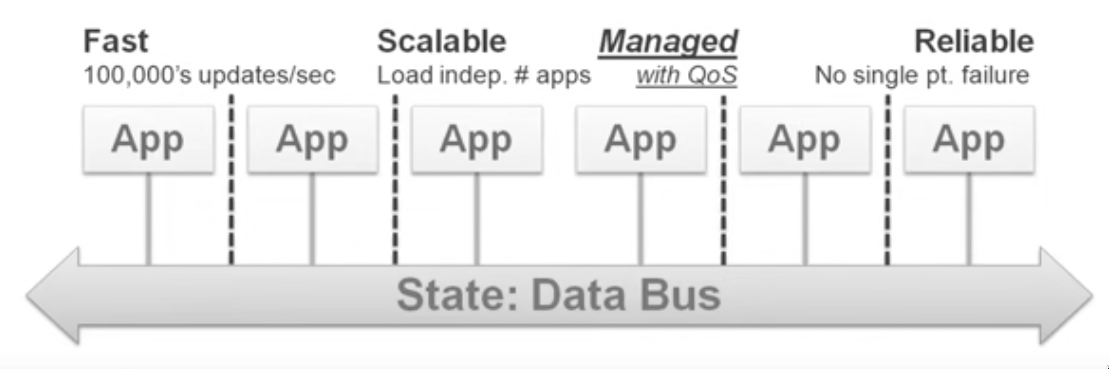
\includegraphics[width=0.6\linewidth]{images/dds-architecture.png}
    \caption{Data Distributed System architecture in a nutshell.}
    \label{fig:dds-architecture-nutshell}
\end{figure}


\subsection{ROS2-DDS Architecture}

As previously stated, the \textit{Robot Operating System 2} was developed to address the former architecture lack of support for real-time systems, mainly due to its architecture design that relied on their own middleware specification. To address this, ROS2 middleware approach is built upon the DDS framework \cite{maruyama2016exploring}, leveraging DDS for its messaging architecture, where communication and transport configuration are handled. 

As far as dependencies are concerned, DDS implementations have light sized dependencies, often related to language implementation libraries, easing the complexity behind installing and running dependencies \cite{ros-on-dds}.

The middleware's on-top layer regards the ROS client library (\textit{rcl}), already implemented in the former ROS architecture. This layer accounts the availability of ROS concepts to the Application layer, as it provides APIs to ease the software implementation by ROS developers \cite{ros2documentation}. As ROS aims to support different programming languages over the same computing context, each language-specficic API must have its corresponding client library (\textit{rclcpp} regarding \textit{C++} and \textit{rclpy} regarding \textit{Python}). The \textit{rcl} accounts these client libraries by abstracting their specification, consequently reducing code duplication \cite{rcl, casini2019response}.

\begin{figure}[H]
    \centering
    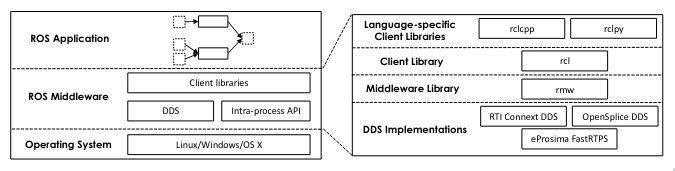
\includegraphics[width=\linewidth]{images/ros2-architecture.png}
    \caption{ROS2 framework architecture.}
    \label{fig:ros2-architecture}
\end{figure}

Towards supplying a wide range of configurations back to application layer, ROS2 aims to support multiple DDS implementations, in which these implementations API specification might differ from each other (currently, \textit{FastRTPS} by \textit{eProsima}, \textit{Connext} by \textit{RTI}, and \textit{Vortex OpenSplice} by \textit{Adlink}). It should be noted that the DDS implementations are low-level of abstraction, strictly defined by its corresponding vendor's API. DDS only defines fundamental procedures at a higher degree of abstraction.  

In order to abstract \textit{rcl} from the specifications complexity of these implementations APIs, an DDS-agnostic interface is being introduced, the \textit{rmw} (ROS MiddleWare) interface \cite{casini2019response}, allowing portability among DDS vendors, which consequently enables ROS developers to interpolate DDS implementations, based on their applications needs during runtime. The information flow through the middleware layer is done over structure mapping between ROS and DDS data models, addressed by the \textit{rmw}, regarding the DDS implementation that is being considered at runtime.

\subsection{Computation Graph}

From a logical perspective \cite{casini2019response}, ROS applications are composed of many software modules that operate as computation nodes, allowing its participation into the ROS \textit{Global Data Space}. The use of publish-subscribe model approach as communication type, through \textit{message-passing} patterns, confers additional concept complexity to the application architecture, where the latter can be naturally represented as a \textit{computation graph} \cite{cousins2010welcome}.

The application's computation graph presents itself as a graphical network, where runtime named entities have their unique role when it comes to data distribution.

\subsubsection{Node Instances}

The application development is done over package orchestrating, where each logically represents a useful software module. Packages might be compromised by numerous \textit{nodes}, that can be perceived as processes that will likely perform computation over the network. It is worth mentioning that, nodes can be connected within a single package or between multiple packages, as they are built over their corresponding packages \cite{cousins2010welcome, intro-ros}.

Thus, the network is comprised by many nodes, running simultaneously and exchanging data between them, where each node addresses its corresponding network module purpose \cite{ros2documentation}. Fault tolerance features are guaranteed as nodes have their corresponding unique name, allowing communication in an unambiguous manner, which confers a suitable approach when developing a complex robotic system.

The notable usage of callback functions provide great functionality when it comes to manage node's behaviour in the communication process. Additionally, \textit{timers} can also be used, since they provide a useful way of managing these callbacks, by time-assigning.

\subsubsection{Communication}

Message-passing is the primary means by which nodes communicate with one another. The \textit{message} definition is a well-typed data structure, which commonly characterizes every data structure concerning the information exchange between nodes. A message is defined by its data type, also known as its \textit{interface}, which can either be primitive (\textit{integer}, \textit{string}, \textit{boolean}, among others), or defined by a complex data structure, where multiple data types are assigned to their corresponding variables \cite{ros2documentation, intro-ros}.

ROS computation graph provides \textit{3} different ways of establish node communication, those being \textit{Topics}, \textit{Actions} and \textit{Services}. These communication mechanisms have different interfaces, specified in different folders with unique namespaces \cite{ros2documentation}.

The concrete mechanisms
\textit{Topics} are perhaps the most common method, naturally perceived as middle-communication buses, over which messages are passed through. As semantic approach, communication through topics is handled by the publishing-subscribing pattern. A node publishes the message to any number of topics, that are then subscribed by nodes that want to get access to that message. Topics provide a multicast routing scheme, where publish data is casted into the multiple nodes that are subscribed to the topic \cite{casini2019response}.

\begin{figure}[H]
    \centering
    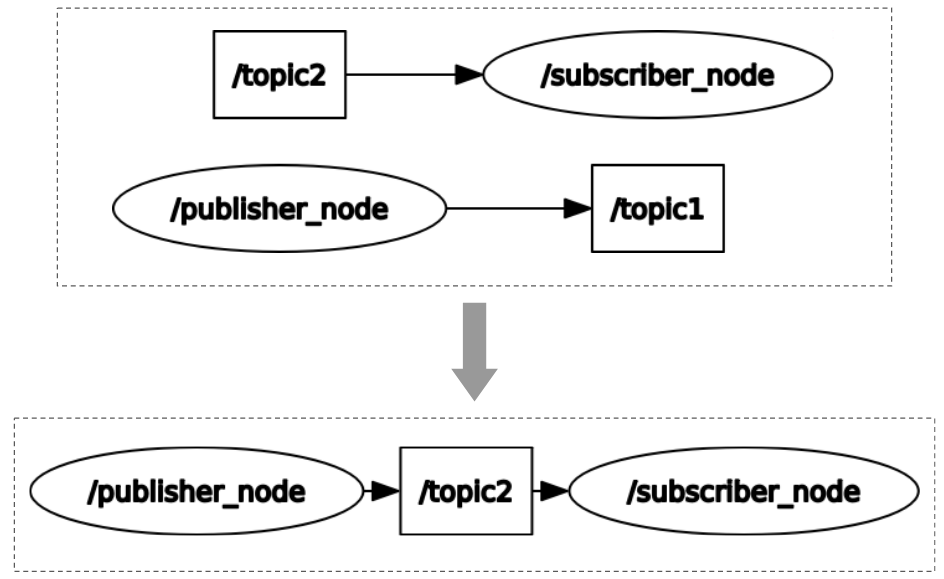
\includegraphics[width=0.5\linewidth]{images/ros2-topics.png}
    \caption{Communication behaviour over \textit{topics}.}
    \label{fig:ros2-topics}
\end{figure}

A specific \textit{topic} is created upon specifying its entity name over either a publisher or a subscriber callback instance. Whenever a node creates a publisher, intentionally instantiated to publish a message through a specified topic, \textit{roscore} is used to advertise the latter, enabling message passing to the corresponding topic subscribers. Message processing is done via the node's callback functions, which are activated upon message receipt, as it can also be utilized for publishing purposes \cite{casini2019response}.

Even though topics are the most conventional way of communication, due to its multicast scheme, subscribers can not be identified by the publishers, so logging and synchronization becomes rather difficult \cite{intro-ros}.

The use of \textit{services} enables a client node, that can also be seen as a topic subscriber, to request data from a server, that likewise a topic publisher, furnish data through a service. This is a bidirectional synchronous form of communication based on a request-response pattern.

Other notable way of exchanging data is by setting goals through \textit{Actions}. Actions are intended to process long-running tasks, where the client sends a goal request to the server node, that confirms the receiving of this goal. The server might provide feedback to the client before providing a response to the client. 


\subsubsection{Launch Files}

A conventional way of deploying a ROS application is through the use of \textit{launch files}, enabling the multi-configuration over entire robotic applications, where network nodes can be individually pre-configurated. Therefore, ROS makes use of the \textit{roslaunch} to automatically initialize the whole network, simultaneously launching each node \cite{intro-ros}. This provides a simpler way of monitoring the system nodes. 

The Figure \ref{fig:ts-rqt-graph} depicts the network architecture corresponding to an ROS application well-known example called the \textit{TurtleSim}. This application is mainly composed by \textit{two nodes}, that perform together towards moving a turtle. Additional nodes were implemented, in order to add complexity to the current network, as to later support security as a proper example. Briefly, the \textit{multiplexer} node acts as a topic selector between two different subscribed topics, where each of them was respectively associated with a priority value. Based on the priority valued, the \textit{multiplexer} node forwards the commands, related to the selected topic, into the \textit{turtlesim} node, triggering the turtle's movement. 

The \textit{rqt} \footnote[1]{ROS provides a GUI tool called \textit{rqt}, that assists developers in manipulating the network elements, in a more user-friendly manner.}, \textit{rqt\_graph}, allows the developer to perform analysis over a graphical visualization of the network computation graph.

\begin{figure}[H]
    \centering
    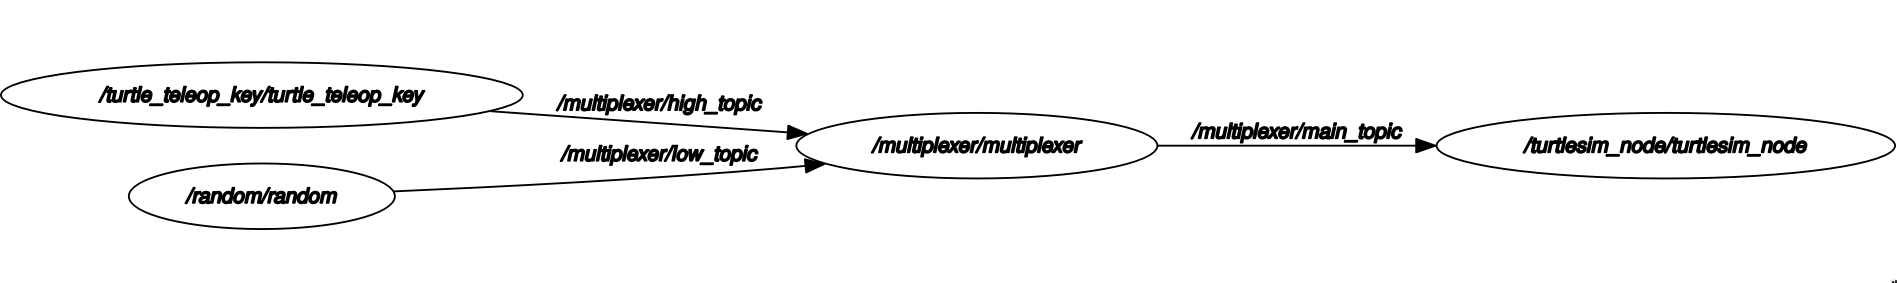
\includegraphics[width=0.8\linewidth]{images/ts_rqt_graph.png}
    \caption{\textit{TurtleSim}'s network graph presented by \textit{rqt\_graph}.}
    \label{fig:ts-rqt-graph}
\end{figure}

After the proper configuration of each node regarding the \textit{TurtleSim} example, the network can be easily managed and automatically launched through a launch file. The Figure \ref{fig:ros-lf} addresses the launch specification related to the latter application.

\begin{figure}[H]
\begin{lstlisting}[otherkeywords={launch, node, name, pkg, exec, output}]
<launch>
    <node name="turtlesim" pkg="default" exec="turtlesim" output="screen"/>
    <node name="keyboard" pkg="default" exec="keyboard"/>
    <node name="random" pkg="random" exec="random"/>
    <node name="multiplexer" pkg="multiplexer" exec="multiplexer"/>
</launch>
\end{lstlisting}
\caption{\textit{TurtleSim} launch file.}
\label{fig:ros-lf}
\end{figure}

Additional node configuration, such as name remapping and parameter adjustments, can be specified under the \textit{args} tag, which offers great functionality to the launching process. 

Distinctive namespaces allow the system to start the nodes, without any name nor topic name conflicts. However, this technique has some flaws attached, since it does not furnish a way of launching nodes in a separated terminal, often needed for user interaction purposes, like input reading.

\subsubsection{Parameters}   

Another relevant concept behind ROS is the existence of nodes \textit{parameters}, that allows individual configuration of the network nodes. In the former version of ROS, the node parameters were controlled by a global \textit{parameter server}, managed by its corresponding ROS Master \cite{intro-ros}. However, in ROS2 each node declares and manages its own parameters, by using the predefined commands \textit{get} and \textit{set}. Additionally, using a parameter function callback, the node's parameters can easily be edited \cite{ros2documentation}.
        
\subsubsection{Node Composition}  

Usually a node is attached to a single process, but it is possible to combine multiple nodes into a single process, structurally abstracting some network parts, while improving the network's performance \cite{ros2documentation}. However, there is a slight difference about how ROS and ROS2 approaches node composition. 

In the former version of ROS, node composition was done over the combination of \textit{nodelets}, intentionally designed to ease the cost of overusing TCP for message-passing between nodes \cite{ros-nodelets}.  Supported by the former idea of \textit{nodelets}, ROS2 introduces the \textit{components} as software code compiled into shared libraries, that can be loaded into a \textit{component container} process at runtime in the network, ensuring node composition \cite{ros2documentation}. 

%Node composition could also be applied for security matters. Suppose a scenario where multiple nodes respect the same security policies. By combining them into a single process, the mapping into this set of rules would be direct, easing the usage of security enclaves.
           

\section{Security}

The deployment of real-time systems implies critical concerning about safety and security \cite{maruyama2016exploring}, resulting of the demanding time-critical scenarios. 

Robotic systems fall under the umbrella of this broad system definition, as they feature unique cyber vulnerabilities related to its integration over highly networked environments, that confers great importance on exposing critical time-reliant scenarios \cite{mcclean2013preliminary, dieber2017security}.

\subsection{Former ROS Security Concerns}

The network security evaluation in a system is done by applying several analyzing techniques. Generally, these techniques do not cover every security aspect, as new vulnerabilities arise from technology evolution \cite{kaeo2004designing}.
The appliance of security countermeasures techniques upon configuring the system's network confers a critical step when aiming towards achieving security.

Within this vast topic, several avenues of endeavor come to mind, each deserving of a substantial study. Network security entails pre-exploration of the system's network through practical networking security techniques, such as intrusion detection and traffic analysis \cite{marin2005network}.

Numerous researchers \cite{8794451, dieber2020penetration} have investigated the use of these techniques, such as port scanning and penetration testing, over the previous version of ROS in order to thoroughly assess attack vulnerability throughout the ROS architecture. 

The ROS Master role in the communication architecture, and its ability to connect to other nodes, imposes many concerns about how to address security to ensure protection over the Master node. Exposing this node poses a critical threat over the whole network \cite{8794451}. 

Moreover, there were also worries regarding the way ROS handled node communication. Network security may be jeopardized, as a result of the publish-subscribe pattern transparency, where node-to-node communications are settled in plain text, making data content vulnerable to unauthorized usage \cite{kim2018security}.
 
However, due to the high non-linearity and complexity of real-time systems, implementing such thorough analysis method in near real-time remains a significant difficult task \cite{diao2009design}.

\subsection{DDS-Security Specification}

The \textit{Object Management Group} (OMG) \cite{3} accounts security integration by supplying an in-depth specification, consequently adding features to the already developed DDS standard. The \textit{DDS-Security} is a specification that serves as a security extension to the DDS protocol, defined by a set of plugins (Authentication, Access Control, Cryptographic, Logging, Data Tagging), combined in a \textit{Service Plugin Interface (SPI)} architecture \cite{8442103, ros-dds-integration}.

\begin{figure}[H]
    \centering
    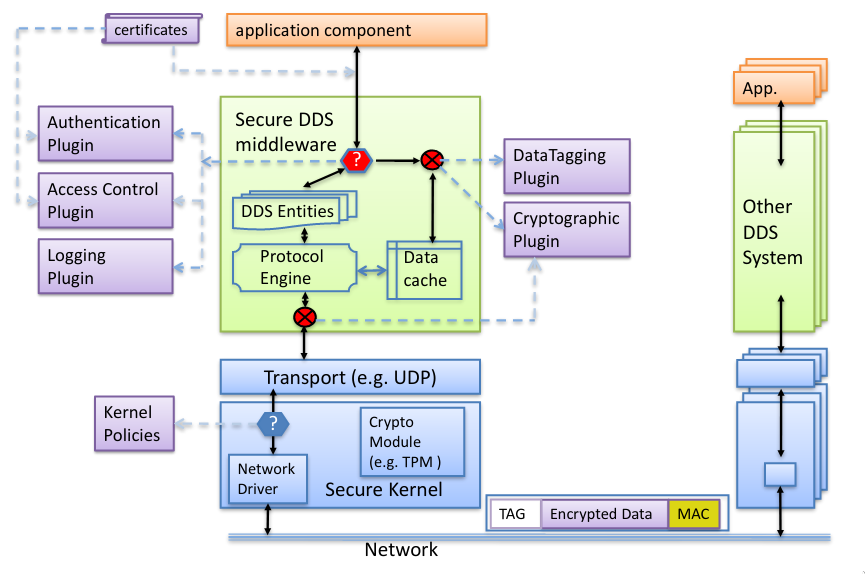
\includegraphics[width=0.7\linewidth]{images/dds-security-architecture.png}
    \caption{DDS-Security Architecture. Extracted from \cite{dds-s}.}
    \label{fig:dds-security-architecture}
\end{figure}

This specification enables its integration by furnishing a \textit{Security Model} supplied to the DDS standard, whereas the \textit{Service Plugin Interface} architecture is responsible for granting plugin enhancement for compliant DDS implementations. Moreover, depending on the security requirements needed for a particular application, these plugins might be adjusted by the latter's runtime DDS implementation \cite{dds-s}.

\subsubsection{Authentication}

Upon considering a secure environment over the DDS \textit{Global Data Space}, data integrity can not be prone to unauthorized usage. Therefore, data exchange requires verification procedures to properly identity the authenticity each DDS domain participant.

The Authentication plugin confers the most valued plugin to the entire SPI architecture, as it provides means to validate the identity of the application, later regarded as a domain participant \cite{dds-s, ros-dds-integration}. 

Each participant must be authenticated prior to entering the data space \cite{white2019network}. Therefore, participants are presented to the secured environment regarding the Public Key Infrastructure (PKI). This latter is in charge of issuing a public certificate, accountable and signed by a trusted certificate authority (CA) \cite{white2019network, white2016sros, ros-dds-integration}. 

The communication establishment over different participants must be preceded by a mutual handshake, where certificates are exchanged to guarantee their authenticity \cite{white2019network, kim2018security}. Additionally, the DDS permissions of a domain peer are also concerned within this handshake. The control over permission distribution is respectively handled by the Access Control plugin.

\subsubsection{Access Control}

As aforementioned, the defined DDS specification handles policy control over the DDS domain through the Access Control plugin, where authenticated parties respective operations are imposed by policy restrictions \cite{dds-s, white2019network}. DDS-related capabilities, that concern domains within the \textit{Global Data Space}, are either assigned or restricted to those authenticated participants \cite{ros-dds-integration}. 

Authenticated participants must be granted access to certain domains, where their roles on data transportation must be accordingly accounted by access permissions. If a participant is perceived as a domain data publisher, the domain restrictions must provide publishing privileges to its data topic \cite{white2019network}. 

Following the authentication procedure, domain authorization is also concerned using the proven Public Key Infrastructure (PKI) \cite{ros-dds-integration}, by embedding policy definitions through certificate extensions \cite{white2016sros}. 

Furthermore, the Access Control plugin employs \textit{2} configuration documents that are allocated to each participant \cite{white2019network}. This provides significant security capability, which is given as a supplement to the authentication procedure.

\textbullet\ Domain Governance: \textit{XML} document defining the domain's security policy.

\textbullet\ Participant Permissions: \textit{XML} document containing the permissions assigned to a given domain participant.

Notably, these configuration files are signed by a trusting Certificate Authority (CA) \cite{ros-dds-integration}. Its corresponding permissions certificate confers protection against elevation of privilege attacks. Therefore, if the policy integrity is jeopardized, the handshake between authenticated parties fails to commence \cite{white2016sros}.

\subsubsection{Communication and Encryption}

% The DDS-Security specification ensures encryption and authentication using \textit{OpenSSL}, while accounting security functions based on encryption standards \cite{takemoto2019performance}. Accordingly, it implements a handshake-based standard, concerning the \textit{OpenSSL} protocols, \textit{Secure Sockets Layer} (SSL) and \textit{Transport Layer Security} (TLS), which are used respectively used to ensure encryption over the network communication \cite{white2016sros, kim2018security}.

%The handshake is used to achieve mutual authentication within participants over the DDS domain. As stated, each participant must be authenticated prior to entering the data space \cite{white2019network}. Therefore, participants are presented to the secured environment regarding the Public Key Infrastructure (PKI). This latter is in charge of issuing a public certificate, accountable and signed by a trusted certificate authority (CA) \cite{white2019network, white2016sros}.

The DDS-Security specification ensures encryption and authentication using \textit{OpenSSL}, while accounting security functions based on encryption standards \cite{takemoto2019performance}. 

Accordingly, it implements a handshake-based standard, concerning the \textit{OpenSSL} protocols, \textit{Secure Sockets Layer} (SSL) and \textit{Transport Layer Security} (TLS), which are used respectively used to ensure encryption over the network communication \cite{white2016sros, kim2018security}. The handshake is used to achieve mutual authentication within participants over the DDS domain \cite{white2019network}.

Following the public key assignment, the \textit{Diffie-Hellman} key exchange protocol properly accounts the mentioned handshake, allowing both participants to exchange data over a shared secret key, while accounting their own public certificate information \cite{kim2018security}. The \textit{rcl} is capable of handling this DDS security requirement, levering ROS-based applications to support SROS2, accounting nodes as authenticated participants \cite{white2016sros}. 

As communication establishment is duly achieved throughout this handshake process, the DDS-Security specification takes advantage of the \textit{AES-GCM} encryption standard concerning data encryption over the implicit channel \cite{kim2018security, takemoto2019performance}.

\begin{figure}[H]
    \centering
    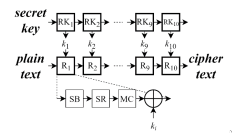
\includegraphics[width=0.4\linewidth]{images/ros_aes.png}
    \caption{\textit{Advanced Encryption Standard} algorithm. Extracted from \cite{takemoto2019performance}.}
    \label{fig:ros_aes}
\end{figure}

The \textit{key cryptosystem} algorithm \cite{takemoto2019performance} presented in the \textit{Advanced Encryption Standard (AES)} considers the usage of functions towards achieving data encryption over the established communication. 

Here, the algorithm combines the shared key established with the message passed over the secure channel. Moreover, it is desirable to implement the \textit{Galois MAC (AES-GMAC)} encryption algorithm, that is based on block cipher operations, consequently adding encryption functionality to the AES algorithm, through a \textit{Message Authentication Code (MAC)} encryption function \cite{takemoto2019performance, kim2018security}.

\subsection{Security Integration in ROS2}

As result of the \textit{Data Distribution Service} (DDS) implementation as a flexible middleware interface in the ROS2 architecture, issues regarding security is no longer mainly ROS-dependent. Thus, when it comes to addressing security over communication, and subsequently data protection enhancement, ROS2 is heavily reliant on how the DDS standard is able to manage security \cite{kim2018security, 8794451}.

Every DDS implementation supported by ROS2 makes use of the DDS-Security specification, enabling security over ROS's application environment. Even though ROS2 is deployed without security mechanisms by default \cite{ros-dds-integration}, ROS2 provides a toolset, the \textit{Secure Robot Operating System 2} (SROS2) toolset \cite{sros2-gh}, extending ROS2's functionality to make use of the DDS-Security functionality. 

The control over these tools are done by \textit{rcl}, providing security over the Application layer, while DDS is capable of providing security over the communication architecture \cite{kim2018security}. SROS2 configuration is done over applying a set of security files to each ROS2 participant, with regard to how DDS handles certificate assignment to their participants \cite{white2016sros}.

The variety of capabilities in SROS2 toolset attempts to aid with security configuration across environments \cite{ros-dds-integration}. However, managing certificates and access control policies might lead to improper configuration. Additionally, orchestrating a real-time network towards achieving a secure environment confers to be a demanding process \cite{ros-dds-integration, white2019network}.

% The SROS2 configuration is done over applying a set of security files to each ROS2 participant, with regard to how DDS handles certificate assignment to their participants \cite{white2016sros}. The variety of capabilities in SROS2 toolset attempts to aid with security configuration across environments, however, the developer must be aware of improper configuration, that can still lead to security problems \cite{ros-dds-integration}.

\subsubsection{Security Enclaves}

The authentication process within the ROS network relies on the notion of a network enclave. Conceptually, an enclave is a secure region in the application address space that maintains confidentiality and integrity, while computations are being carried out on data.

As aforementioned, ROS2 relies on how handles DDS security over their \textit{Domain Participants}. DDS imposes the authentication of each participant prior to joining its \textit{Global Data Space} \cite{white2019network}.

Accordingly, ROS2 ensures authentication over nodes by conceiving the idea of security enclaves, where security artifacts are stored to properly achieve security over the network data space \cite{ros-security-enclaves}. Recall that, these artifacts are implicitly concerned by DDS-Security specification, where the Certificate Authority and an established Public Key Infrastructure (PKI) comes in hand \cite{white2019network, white2016sros}. 

Previously, a node was perceived as a separated DDS participant. However, by considering node composition as a reliable way of matching multiple nodes simultaneously to the same security domain, this node perception as participants can not be taken into account, due to causing non-negligible overhead, as memory space becomes rather difficult to handle \cite{ros-security-enclaves, ros-access-control}.

Concerning the enclave authentication procedure, its security artifacts must be addressable by a DDS participant, where the latter matches to a node sharing context \cite{ros-security-enclaves}.
 
\vspace{0.5cm}
\textbf{Access Control within Enclaves}

Following the \textit{ConArmor} policy language \cite{white2018procedurally}, the SROS2 toolset offers a \textit{XML schema}, where security policies bind profiles to access permissions for network objects, granting privileges back to a certain profile. \textit{Profiles} are implemented under the \textit{enclave} declaration, to duly support the node composition into a single process, enabling the possibility of combining multiple profiles, respectively addressing its corresponding node. Typically, each \textit{enclave} declaration is linked to a corresponding ROS node, naturally perceived as a DDS participant.

\textit{Objects} are classified over a subsystem type, structurally characterized by permissions tags. Then \textit{object privileges} are controlled over access values, either \textit{allow} or \textit{deny}, attributed to their corresponding permissions tags \cite{ros-access-control}. The policy design approach works under the \textit{Mandatory Access Control} (MAC), that denies any privilege by default. The only way of allowing access to any object, is by explicitly specifying the subject's privilege access \cite{ros-access-control, white2018procedurally}.

Depicted in the Figure \ref{fig:ros-access-file}, it is presented a policy file where access control privileges are distributed across enclaves, and their inherited profiles. Recall the \textit{TurtleSim} example, the following \textit{XML} policy file addresses the access to topics for each respective enclave. 

\begin{figure}[H]
\begin{lstlisting}[otherkeywords = {xml, version, encoding, policy, version, enclave, enclaves, profile, profiles, topic, topics, service, services, action, actions, xmlns:xi, path, ns, node, publish, subscribe, reply, request, call, execute}]
<?xml version="1.0" encoding="UTF-8"?>
<policy version="0.2.0"
  xmlns:xi="http://www.w3.org/2001/XInclude">
  <enclaves>
    <enclave path="/">
      <profiles>
        <profile ns="/" node="default">
          <topics publish="ALLOW" subscribe="ALLOW">
            <topic>/*</topic>
          </topics>
          <services reply="ALLOW" request="ALLOW">
            <service>/*</service>
          </services>
          <actions call="ALLOW" execute="ALLOW">
            <action>/*</action>
          </actions>
        </profile>
      </profiles>
    </enclave>
  </enclaves>
</policy>
\end{lstlisting}
\caption{SROS2 policy file regarding the access control policies over the \textit{TurtleSim} example.}
\label{fig:ros-access-file}
\end{figure}